\documentclass[12pt]{article}
\usepackage{graphicx}
\usepackage{mathabx}
\usepackage{todonotes}
\usepackage{algorithm}
\usepackage{algpseudocode}
\begin{document}
    \title{Focused Reading Tech Report}
\author{Enrique Noriega}
\date{\today}
\maketitle
\pagebreak

\section{Use Case}
\label{sec:usecase}
We want to find details about the interaction of two elements of a model. For
example, how does mTOR interacts with cell apoptosis. A biologist may have existing knowledge, like the DyCE model, where existing high level interactions are described, which are already digested. Our experiment focuses on finding lower level details about these interactions by reading the literature (PMC OA) by the means of a Reinforcement Learning process.

\section{Modeling Details}
\label{sec:modeling}
We represent a biological model as a directed graph, where vertices represent  participants in chemical reactions, like proteins, genes or other gene products or higher level biological processes, like apoptosis. 

Edges represent an interaction, which comes from any event extracted by REACH. The direction of the edges goes from the cause of the event to its theme.

Edges are also labeled. The label is the sign of an interaction. A positive sign means that the cause promotes the theme and a negative sign means that the cause inhibits the theme.

Information extracted by REACH is used to compose the directed graph. Where the story of how Participant A interacts with Participant B is described by the path or paths connecting them together.

\section{Problem Description}
\label{sec:problemdesc}
We start with a graph with only to vertices and no edges. The vertices are the source and the destination of the search. An example of these elements are mTOR and apoptosis, as in the use case.

To find information that can potentially link together both vertices, we perform a Lucene query over the open access. Details for the query are described on Appendix \ref{apx:query}. The query returns a set of documents likely to contain an interaction where both elements are participants on an IE event. The returned documents are fed to REACH, and the extracted information is reconciled into the model graph in the form of new vertices and edges.

If there is a directed path connecting the source and the destination, this path becomes the explanation of how they interact. Although this is possible, it’s unlikely that it will be the case in general.


If there exist no such path, the source and destination will be on different connected components. When this situation arises, we enter into an iterative phase, where we increase the information in the model by growing the graph. 

We use two strategies to grow it:
\begin{enumerate}
  \item \textbf{Exploration}: Do information retrieval and extraction to fetch documents that are likely to increase the number of vertices in the graph.
  \item \textbf{Exploitation}: Do the same with the goal of increasing the radius of the components. The radius is defined as the length of the longest directed path in a component.
\end{enumerate}

Both queries operate pair-wise where we provide two participants: $X$ and $Y$. Remember that a participant is represented by a vertex in the graph. The set of possible $(X,Y)$ pairs is the cross product of the connected components.

\begin{figure}[hbt]
  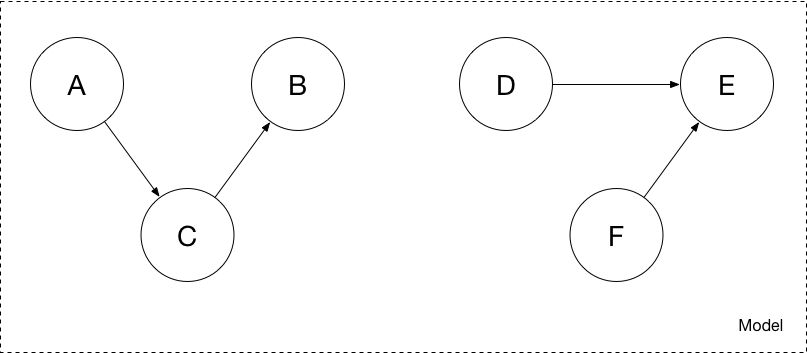
\includegraphics[width=\textwidth]{model.png}
  \caption{A grown model with six participants}
  \label{fig1}
\end{figure}


The possible pairs from the graph in Figure \ref{fig1} are: 

\begin{equation}
  \{(A,D), (A,E), (A,F), (B,D), (B,E), (B,F), (C,D), (C,E), (C,F)\}
\end{equation}


Some of the pairs are better suited for introducing more elements to the model and some other pairs are better suited for finding elements that connect independent components together. Details on how to estimate this will be described further down.

\section{Reinforcement Learning Setup}
\label{sec:rl}

\subsection{Intuition}
The goal of casting the problem into a RL setup is to \emph{do the most spending the least}. Searching for information about the correct elements in the model are more likely to lead us to find new elements that could be in a path between the source and the destination of the search. A \emph{cost} we pay is \emph{reading}. Theoretically we can read all the documents in \emph{PMC OA} and have all the information available in the literature, but the repository consists of more than a million scientific articles, and most of them aren't related to our focused search.

Instead, depending on the current state of the model at any given time of the search, we hypothesize that the RL agent learns a policy that guides the search by selecting the best elements in the model to achieve the goal of the search.

We will define the building blocks of the RL setting based in the modeling introduced in section \ref{sec:modeling}.

\subsection{Algorithm}
We can formulate the problem at high level as described in algorithm \ref{alg:focusedreading}.

\begin{algorithm}
\caption{Focused Reading algorithm}\label{alg:focusedreading}
\begin{algorithmic}[1]
\Procedure{focused\_reading}{$S,D$}\Comment{$S$ and $D$ are the src and dst}
   \State $G \gets \{\}$ \Comment{$G$ holds the model as a graph}
   \Repeat
		\State $(A,B) \gets $ \Call{ChooseEndPoints}{$S,D,G$} \label{alg:chendpoints}
   		\State $Q \gets$ \Call{ChooseQuery}{$A,B,G$}	\label{alg:chquery}
   		\State $(V, E) \gets$\Call{Lucene+Reach}{$Q$}\Comment{Query and IE}
   		\State \Call{Expand}{$V, E, G$}\Comment{Add the new elements to the model}
   \Until{\Call{IsConnected}{$S,D$} OR \Call{StopConditionMet}{$G$}}
\EndProcedure
\end{algorithmic}	
\end{algorithm}

Special details are deserved for two calls in the pseudocode.

\begin{itemize}
  \item \emph{ChooseEndPoints} (alg \algref{alg:focusedreading}{alg:chendpoints}):\\
 		Is the strategy followed to select the elements of the model which will anchor the next stage of the search. Multiple strategies are being explored to select:
 		\begin{itemize}
			  \item \emph{PageRank}: PR is a ranking algorithm that orders the elements of a network by how likely is to visit an element in the long term. Which of the elements in the ranking to pick is still open to discussion. Intuitively, the highest ranked element would be a good element to chose as an anchor for the search, although we could chose some others. The particular candidate choices are:
			  	\begin{itemize}
 					\item Highest ranked participant (Top PR element)
 					\item Lowest ranked participant (Inverse of the top PR)
 					\item Element at the middle of the ranking.
				\end{itemize}

			  \item \emph{TF-IDF}: This is another ranking metric. Functionally, the same argument as with PR holds with TF-IDF, the difference is that in order to order the elements, it uses collection the frequency and the document frequency. The highest ranked element by tf-idf will, more or less be the element with the highest frequency in the Open Access normalized by the inverse of the number of articles where it appears.
			  \item \emph{Most recently added element(s)}: Select the most recently added element or elements of the model. It is likely that the amount of these class of nodes is very large, hence we might need to rank these as well and take one of the elements.
			  \item \emph{PMI}: Point-wise mutual information quantifies how likely are we to see together two elements in a collection. Using PMI we rank all the candidate endpoints relative to another element, for example, the search's source or destination and picke that with the highest probability.
		\end{itemize}

  \item \emph{ChooseQuery}(alg \algref{alg:focusedreading}{alg:chquery}): Multiple query strategies will be used to trade exploration and exploitation. 
		\begin{enumerate}
		  \item \emph{Same document with distance constraint}: This is a family of queries, where we retrieve all documents that contain both elements within the certain number of tokens. The number of tokens is a parameter and it's variated to create the family of query strategies.
		  \item \emph{Same document without distance constraint}: This query strategy retrieves documents where both participants are present, but doesn't put any constraint in their distance.
		  \item \emph{Any document containing}: Documents that contain either of the elements match the query and will be retrieved.
		\end{enumerate}

\end{itemize}




\subsection{Actions}
We introduced two search strategies in section \ref{sec:problemdesc}. To elaborate on how to cast them as actions, first we introduce two functions to use in order to rank the usefulness of a \emph{pair} with respect to both search strategies.

\begin{itemize}
  \item $f_1$: Given participants $X$ and $Y$ the mean of the number of times they appear together in a document $d$ of corpus $D$ in the form of an interaction.  		\begin{equation}
  \label{eq:f1}
  			f_1(X,Y) = average_{d\in D} tf_d(X,Y)
		\end{equation}
		
		\item $f_2$: Given participants $X$ and $Y$ the document $d$ of corpus $D$ with the highest number of interactions in the form of an interaction
		\begin{equation}
		\label{eq:f2}
  		f_2(X,Y) = \arg\max_{d\in D} tf_d(X,Y)
\end{equation}
\end{itemize}

By using equations \ref{eq:f1} and \ref{eq:f2}, we can define two different \emph{action templates}, one per search strategy, which are parameterized.

\begin{itemize}
  \item \textbf{Exploration Action}: Let $P_N$ be the set with the $N$ highest ranked elements in the graph by $f_1$.\begin{equation}
  QExplore_N(P) = top_{N, p \in P} f_1
\end{equation}

  \item \textbf{Exploitation Action}: Let $P_N$ be the set with the $N$ highest ranked elements in the graph by $f_1$.\begin{equation}
  QExploit_N(P) = top_{N, p \in P} f_2
\end{equation}

The \emph{return values} of both action templates are
\begin{equation}
\label{eq:return}
  \{(V,E), M\}
\end{equation}

 The set new vertices and edges, $(V,E)$ to be added to the model graph and $M$, the amount of documents returned by the query. We prefer a query that adds many elements (utility) by reading less papers (cost).

By abstracting the parameter as $N$ as a predefined set, for example $N \in {1,10,100,1000}$, we are reducing the action space to a manageable size, in this particular example to $2 \times 4 = 8$ possible actions.
\end{itemize}


\subsection{Reward function}

If the agent decides to take an \emph{exploration action} at time step $t$, we would prefer that the elements added to the model graph have can be used at a later stage to perform another action. Similarly we make the same argument if the agent decides to take an \emph{exploitation action}. If we have a measure of how suitable is the model graph for exploration and exploitation, we can have a craft a reward function incorporates a measure of how much did it increase or decrease. Consider the set $P$ of all pairs in the model graph; define the following statistics:

\begin{itemize}
  \item \textbf{Exploration score}: Estimates how well suited is the model graph to do exploration by taking the average $f_1$ values of all the possible pairs $p \in P$.
\begin{equation}
\label{eq:exploration-score}
  u(P) = average_{p\in P} f_{1}(p)
\end{equation}
Ideally, a higher $u$ score can lead to further exploration actions that introduce more elements into the model graph.
\item \textbf{Exploitation score}: Estimates how well suited is the model graph to do exploitation by taking the average of the \emph{top N} pairs by $f_2$, contained in set $I$.
\begin{equation}
\label{eq:exploitation-score}
  v(P) = average_{n\in N(P)} f_{2}(n)
\end{equation}
A high $v$ score could lead to the introduction of elements to the model graph that help connect independent components together.

\end{itemize}

Overriding notation a little bit, let $u_t$ be the exploration score of the model graph at epoch $t$. Let $v_t$ be defined similarly for the exploitation score. We define the reward function $R$ as:

\begin{equation}
  R(t) = \Delta u + \Delta v - \alpha M - \beta \rho 
\end{equation}

Where each term has the following meaning:

\begin{itemize}
  \item $\Delta u$: $u_t - u_{t-1}$ Difference in exploration score with respect to the previous epoch.
  \item $\Delta v$: $v_t - v_{t-1}$ Difference in exploitation score with respect to the previous epoch.
  \item $\alpha M$: Amount of documents read during the executed action. Coefficient $\alpha$ is a hyper parameter that must be specified.
  \item $\beta \rho$: Path length \todo{What did we mean by this term?} Coefficient $\beta$ is a hyper parameter.
\end{itemize}

If the action taken was successful, its corresponding delta will be positive, meaning that the graph is better suited for exploration and/or exploitation. If the deltas have a negative sign, means that the model graph is in a worse condition than before taking the action. $M$, as defined in equation \ref{eq:return}, is the cost the process payed to execute the desired action. Ideally we want positive values for the delta temrs and small magnitures for $\alpha M$.

\todo{Say something about $\beta \rho$}

This reward function will be plugged into the \emph{Bellman equation} to be our objective function during learning.

\subsection{State}

The model graph's state will serve as predictors to compute the \emph{q-values}. Let the \emph{radius} of a component in a graph be the length of its longest path. Some of the discussed properties we will use are:

\begin{itemize}
  \item Number of connected components.
  \item Max and average radius of the components
  \item Max and average number of vertices
  \item Max and average \emph{density}
  \item Max and average number of leaves
  \todo{Should we add U and V?}
\end{itemize}

In terms of supervised machine learning, the state are the features we will use to train the \emph{Q function}.

\emph{Q Function}

A regular feed-forward neural network will be used to learn a Q Function. However, we may explore more neural network architectures.

\section{Evaluation}

To evaluate the performance of the agent, we will hold out certain number of interaction paths present in the \emph{DyCE model}. The DyCE model contains summarized pathways. If the agent is able to put together low-level legitimate paths that connect the elements of DyCE together, it will be considered a hit.

To asses the legitimacy of a link, evidence text will be inspected by a human to make sure that it supports the claim made by the automated reader.




\section{Implementation}

This project will be written using Python and Keras to handle efficiently numerical computation, with the option of accelerating computation using the CPU.

Reading PMC OA and querying the Lucene index can by time consuming, but these processes can be executed once and have their results stored. With the \emph{CMU} output files, we can cache the following information in a SQLite or Postgres database:

\begin{itemize}
  \item The set of all entities that are participants of any interaction
  \item The resulting documents of querying a pair of participants
  \item All the different interactions and their frequency in any document
\end{itemize}

With a proper relational design and indexing strategy, searching for this data at any epoch will be significantly more efficient than querying lucene and reading with REACH. \todo{Add a relational diagram of the tables}

\pagebreak
\appendix
\section{Query Algorithm}
\label{apx:query}
\todo{Fill it}
\end{document}